\section{Ejercicio 5: Heurística de búsqueda local}

% Obviamente, el Doc está en desacuerdo y dice que la heurística golosa no es
% la mejor idea. Para justificar su postura les pide diseñar e implementar una
% heurística de búsqueda local para MCS, y desarrollar los siguientes puntos
% para, de una buena vez, convencer a Marty:
% a) Explicar detalladamente el algoritmo implementado. Plantear al menos dos
%    vecindades distintas para la búsqueda.
% b) Calcular el orden de complejidad temporal de peor caso de una iteración
%    del algoritmo de búsqueda local (para las vecindades planteadas). Si es
%    posible, dar una cota superior para la cantidad de iteraciones de la
%    heurística.
% c) Realizar una experimentación que permita observar la performance del
%    algoritmo comparando los tiempos de ejecución y la calidad de las
%    soluciones obtenidas, en función de las vecindades utilizadas y elegir,
%    si es posible, la configuración que mejores resultados provea para el
%    grupo de instancias utilizado.

\subsection{Introducción}
Este ejercicio consiste en la implementación de una heurística de búsqueda
local para el problema de \acr{MCS}, que sea capaz de iterar sobre una
solución dada y mejorarla en búsqueda de óptimos locales.

Al igual que en el ejercicio anterior, asumiremos sin pérdida de generalidad
que los grafos $G_1$ y $G_2$ para los que quiere resolverse el problema son
tales que $N_1 \leq N_2$, siendo $N_1$ y $N_2$ sus cantidades de nodos
respectivas.

\subsection{Vecindades planteadas}

El principal elemento a definir a la hora de plantear una heurística de
búsqueda local es qué soluciones se considerarán vecinas. Es decir, es
necesario plantear una \emph{relación de vecindad} entre el espacio de
soluciones del problema. Para esto, será útil adoptar de nuevo el enfoque
de ver a una solución de \acr{MCS} como un mapeo $s : V(G_1) \to V(G_2)$.
De esta forma, se define el espacio de soluciones posibles del problema como
\[ S = \lbrace s : V(G_1) \to V(G_2) \ \vert\ s \text{ es inyectiva}
\rbrace \]
y se plantean dos alternativas para definir una relación simétrica $N
\subseteq S \times S$.
Luego, dada una solución del problema $s \in S$, la heurística
explorará todas las soluciones vecinas de $s$, es decir, aquellas que se
relacionen con $s$ a través de $N$.

Una característica que se tuvo en cuenta a la hora de definir las vecindades
fue que cualquier solución fuera alcanzable desde cualquier otra, moviéndose
sucesivas veces entre soluciones vecinas.

A continuación se describen las dos vecindades planteadas, junto con el
pseudocódigo del algoritmo que itera sobre cada una de ellas y selecciona,
dada una solución cualquiera, la mejor entre sus soluciones vecinas, y una
estimación teórica de la complejidad temporal de dicha iteración.

\subsubsection{Vecindad $N_1$}
Dos soluciones $s, s' \in S$ se consideran vecinas en la vecindad $N_1$
si $s'$ es el resultado de modificar el mapeo de exactamente uno de los nodos
de $G_1$ en $s$, asignándole un nodo de $G_2$ que esté libre en $s$. Es
decir, $(s, s') \in N_1$ si y solo si
\begin{itemize}
    \item $(\exists \ v \in G_1)\ s(v) \neq s'(v)$, y
    \item $(\forall \ w \in G_1)\ w \neq v \Rightarrow s(w) = s'(w)$.
\end{itemize}

Es importante notar que esta vecindad no está bien definida, y por lo tanto no
puede aplicarse, si $\#V(G_1) = \#V (G_2)$.

\begin{figure}[htbp]
    \centering
    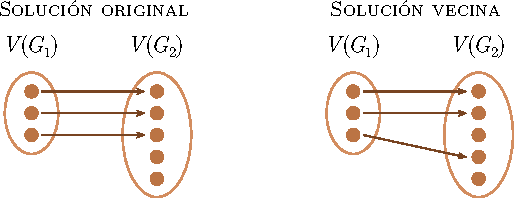
\includegraphics{imagenes/ex5_vecindad1.pdf}
    \caption{Ejemplo de soluciones vecinas que es posible obtener mediante la
    vecindad $N_1$.}
    \label{fig:ej5:vecindad1}
\end{figure}

\noindent\textbf{Pseudocódigo de una iteración}
\bigskip

\begin{algorithm}[H]
    \SetAlgoVlined
    \caption{Iteración de la vecindad $N_1$}
    \Input{Dos grafos $G_1$ y $G_2$, con $\#V(G_1) < \#V(G_2)$, y un tercer
    grafo \textit{solución}, cuyos nodos son pares de $V(G_1) \times V(G_2)$,
    representando la solución a \acr{MCS} que se pretende mejorar. Este último
    grafo será modificado por el algoritmo.}
    \Output{Un valor de verdad indicando si se pudo mejorar la solución.}
    \textit{hay\_mejora} $\gets$ \textsf{falso} \;
    \textit{mejor\_diferencia\_ejes} $\gets$ 0 \;

    \ForEach{vértice $(v, w)$ de \textit{solución}} {
        \ForEach{vértice $w'$ de $G_2$ que no esté en el mapeo} {
            \textit{cant\_aristas\_perdidas} $\gets$ grado de $(v, w)$ en \textit{solución} \;
            \textit{aristas\_nuevas} $\gets$ vector vacío \;
            \ForEach {vecino $\tilde{w}$ de $w_2$ en $G_2$} {
                \If{$\tilde{w}$ está en el mapeo} {
                    $\tilde{v}$ $\gets$ nodo de $G_1$ al que está mapeado $\tilde{w}$ \;
                    \If{$\tilde{v}$ es vecino de $v$ en $G_1$} {
                        agregar $(\tilde{v}, \tilde{w})$ \textit{aristas\_nuevas} \;
                    }
                }
            }
            \textit{diferencia\_aristas} $\gets$ (tamaño de \textit{aristas\_nuevas})
                $-$ \textit{cant\_aristas\_perdidas} \;
            \If{\textit{diferencia\_ejes} $>$ \textit{mejor\_diferencia\_ejes}} {
                \textit{hay\_mejora} $\gets$ \textsf{verdadero} \;
                \textit{mejor\_diferencia\_ejes} $\gets$ \textit{diferencia\_ejes} \;
                \textit{mejor\_para\_eliminar} $\gets$ $(v, w)$ \;
                \textit{mejor\_para\_agregar} $\gets$ $(v, w')$ \;
                \textit{mejor\_aristas\_nuevas} $\gets$ \textit{aristas\_nuevas} \;
            }
        }
    }
    \eIf{\textit{hay\_mejora}} {
        eliminar el nodo \textit{mejor\_para\_eliminar} de \textit{solución} \;
        agregar el nodo \textit{mejor\_para\_agregar} a \textit{solución} \;
        \ForEach{par $(\tilde{v}, \tilde{w})$ en \textit{aristas\_nuevas}} {
            agregar en \textit{solución} una arista entre
                \textit{mejor\_para\_agregar} y $(\tilde{v}, \tilde{w})$ \;
        }
        \Return{\textsf{verdadero}}
    } {
        \Return{\textsf{falso}}
    }
\end{algorithm}
\bigskip

% Complejidad temporal

\subsubsection{Vecindad $N_2$}
Dos soluciones $s, s' \in S$ se consideran vecinas en la vecindad $N_2$
si $s'$ es el resultado de aplicar sobre $s$ alguno de estos cambios:
\begin{itemize}
    \item \textsc{Permutación:} permutar los mapeos de dos nodos de $G_1$, de
    forma tal que $s'(v_1) = s(v_2)$ y $s'(v_2) = s(v_1)$. Formalmente,
    \begin{itemize}
        \item $(\exists \ v_1, v_2 \in G_1)\ s'(v_1) = s(v_2)$ y $s'(v_2) = s
        (v_1)$, y
        \item $(\forall \ w \in G_1)\ w \neq v_1$ y $w \neq v_2
        \Rightarrow s(w) = s'(w)$.
    \end{itemize}
    \item \textsc{Intercambio:} la misma operación que define la vecindad
    $N_1$, es decir, modificar el mapeo de exactamente uno de los nodos
    de $G_1$, asignándole un nodo de $G_2$ que esté libre en $s$. Formalmente,
    \begin{itemize}
        \item $(\exists \ v \in G_1)\ s(v) \neq s'(v)$, y
        \item $(\forall \ w \in G_1)\ w \neq v \Rightarrow s(w) = s'(w)$.
    \end{itemize}
\end{itemize}

La vecindad $N_2$ no tiene problemas de definición en el caso de que $\#V(G_1)
= \#V (G_2)$.

\begin{figure}[htbp]
    \centering
    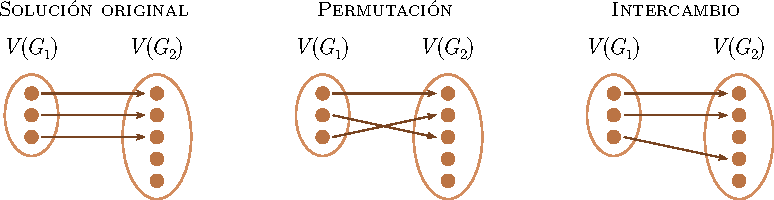
\includegraphics{imagenes/ex5_vecindad2.pdf}
    \caption{Soluciones vecinas que es posible obtener mediante la vecindad
    $N_2$.}
    \label{fig:ej5:vecindad2}
\end{figure}

Cabe destacar que la vecindad $N_1$ está contenida en la vecindad $N_2$,
siendo esta última considerablemente más grande. Desde un punto de vista
computacional, esto tiene como desventaja inmediata un mayor costo a la hora
de recorrer y explorar la vecindad, pero corre con la ventaja de que resulta
posible pasar de una solución dada a cualquier otra en una cantidad de
iteraciones menor (se puede decir que $N_2$ es una vecindad más
\emph{densamente conectada} que $N_1$).

% Pseudocódigo de una iteración

% Complejidad temporal

\subsection{Implementación}

\subsection{Experimentación}
